

\documentclass{beamer}
\title{Advanced Systems Lab - Design} 
\author{Lukas Elmer, Matthias Ganz} 
\date{\today} 

\usepackage{epstopdf}



%\usetheme{Antibes}
%\usecolortheme{default}


\begin{document}

%%%%%%%%%%% SLIDE %%%%%%%%%%%%%%%

\begin{frame}
\titlepage
\end{frame} 

%%%%%%%%%%% SLIDE %%%%%%%%%%%%%%%

%\begin{frame}
%\frametitle{Table of content}
%\tableofcontents
%\end{frame} 

%%%%%%%%%%% SLIDE %%%%%%%%%%%%%%%

\section{Design Choices}
\begin{frame}
\frametitle{Design Choices}

\begin{itemize}
\item The messaging system utilizes a single database instance. 
\item On the logic tier multiple middleware instances may be running. 
\item A client connects to a single middleware.
\item{Every client has a private queue where he can receive private messages}

\end{itemize}

\end{frame}

%%%%%%%%%%% SLIDE %%%%%%%%%%%%%%%


\section{Overview}
\begin{frame}
\frametitle{System Overview}

\begin{figure}
  \begin{center}
    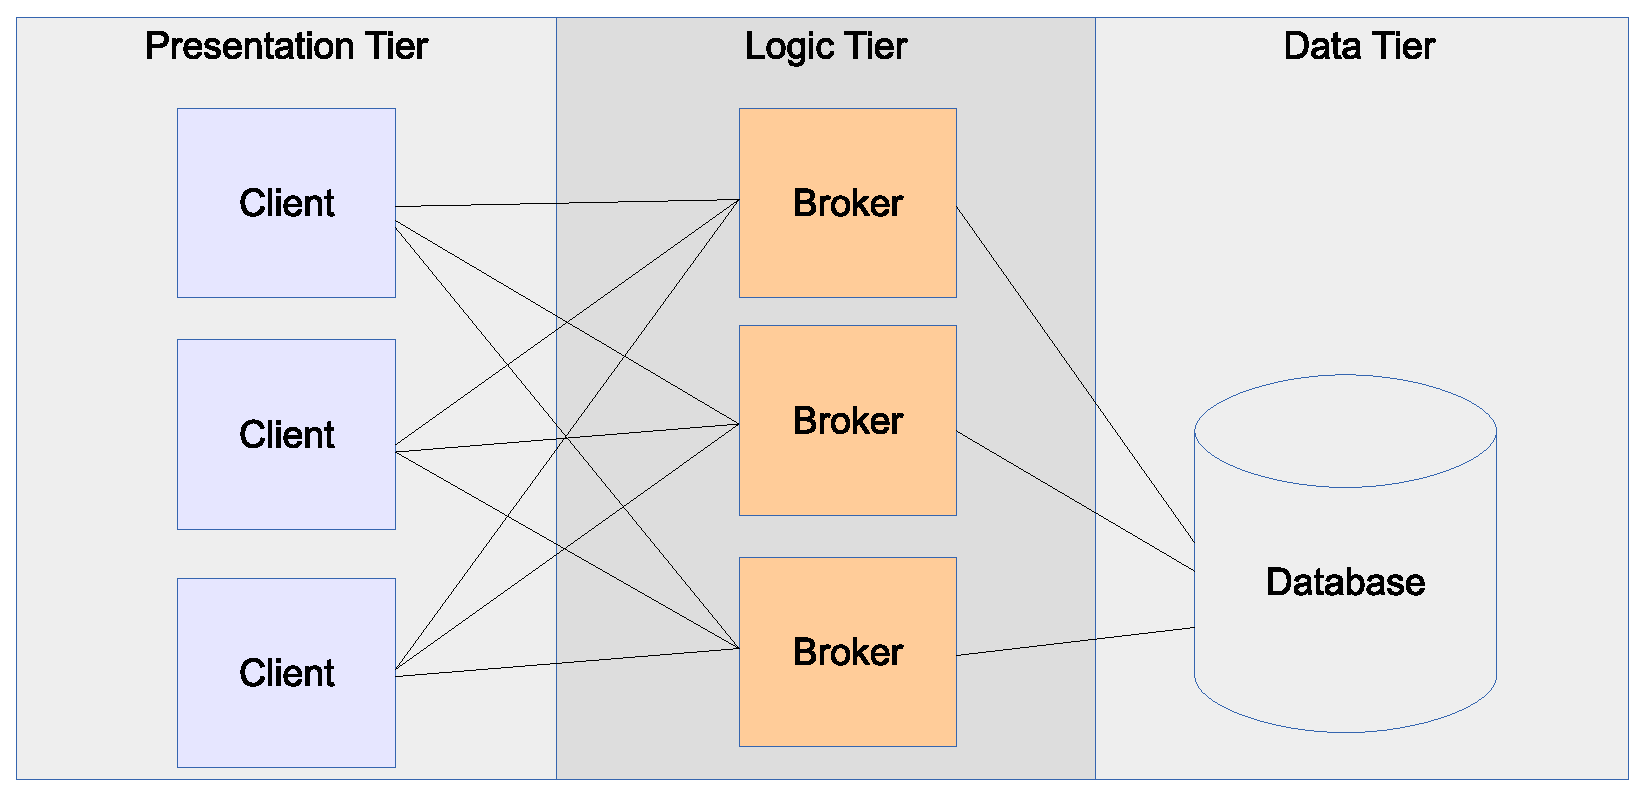
\includegraphics[scale=0.4]{../../drawings/system-overview.eps}
  \end{center}
  \caption{System Overview}
  \label{fig:system-overview}
\end{figure}


\end{frame}

%%%%%%%%%%% SLIDE %%%%%%%%%%%%%%%

\section{Messaging System}

\begin{frame}
\frametitle{Middleware Threading}
\begin{figure}
  \begin{center}
    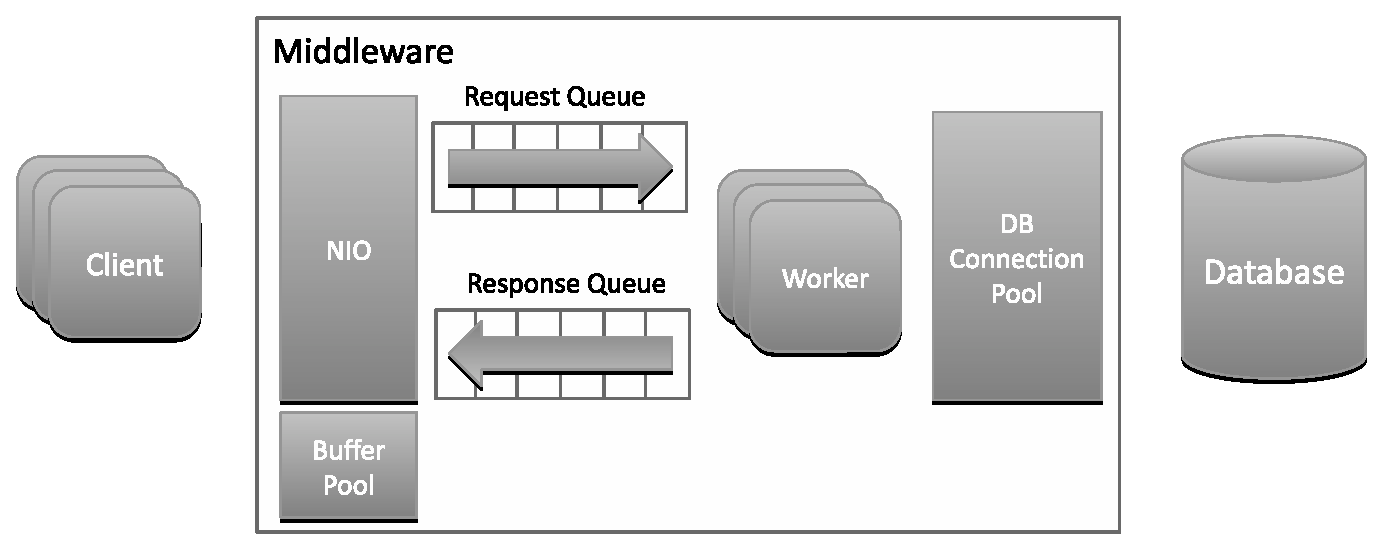
\includegraphics[scale=0.4]{../../drawings/broker-threading.eps}
  \end{center}
  \caption{Middleware Threading}
  \label{fig:middleware-threading}
\end{figure}

\end{frame}

%%%%%%%%%%% SLIDE %%%%%%%%%%%%%%%


\section{Database}
\begin{frame}
\frametitle{Database Schema}

\begin{figure}
  \begin{center}
    \includegraphics[scale=0.6]{../../database/db-schema.png}
  \end{center}
  \caption{Database Schema}
  \label{fig:db-schema}
\end{figure}
\end{frame}

%%%%%%%%%%% SLIDE %%%%%%%%%%%%%%%

\begin{frame}
\frametitle{Client to Broker Communication}

\begin{itemize}
\item Request/Response communication
\begin{itemize}
\item Header: Length of the Java object in bytes.
\item Body: Serialized Java object (Request, Response).
\item Serialize POJO's and send it over the network
\end{itemize}

\item Connection: keep alive
 
\end{itemize}
\end{frame}

%%%%%%%%%%% SLIDE %%%%%%%%%%%%%%%

\begin{frame}
\frametitle{Experiment Setup}
\begin{figure}
  \begin{center}
    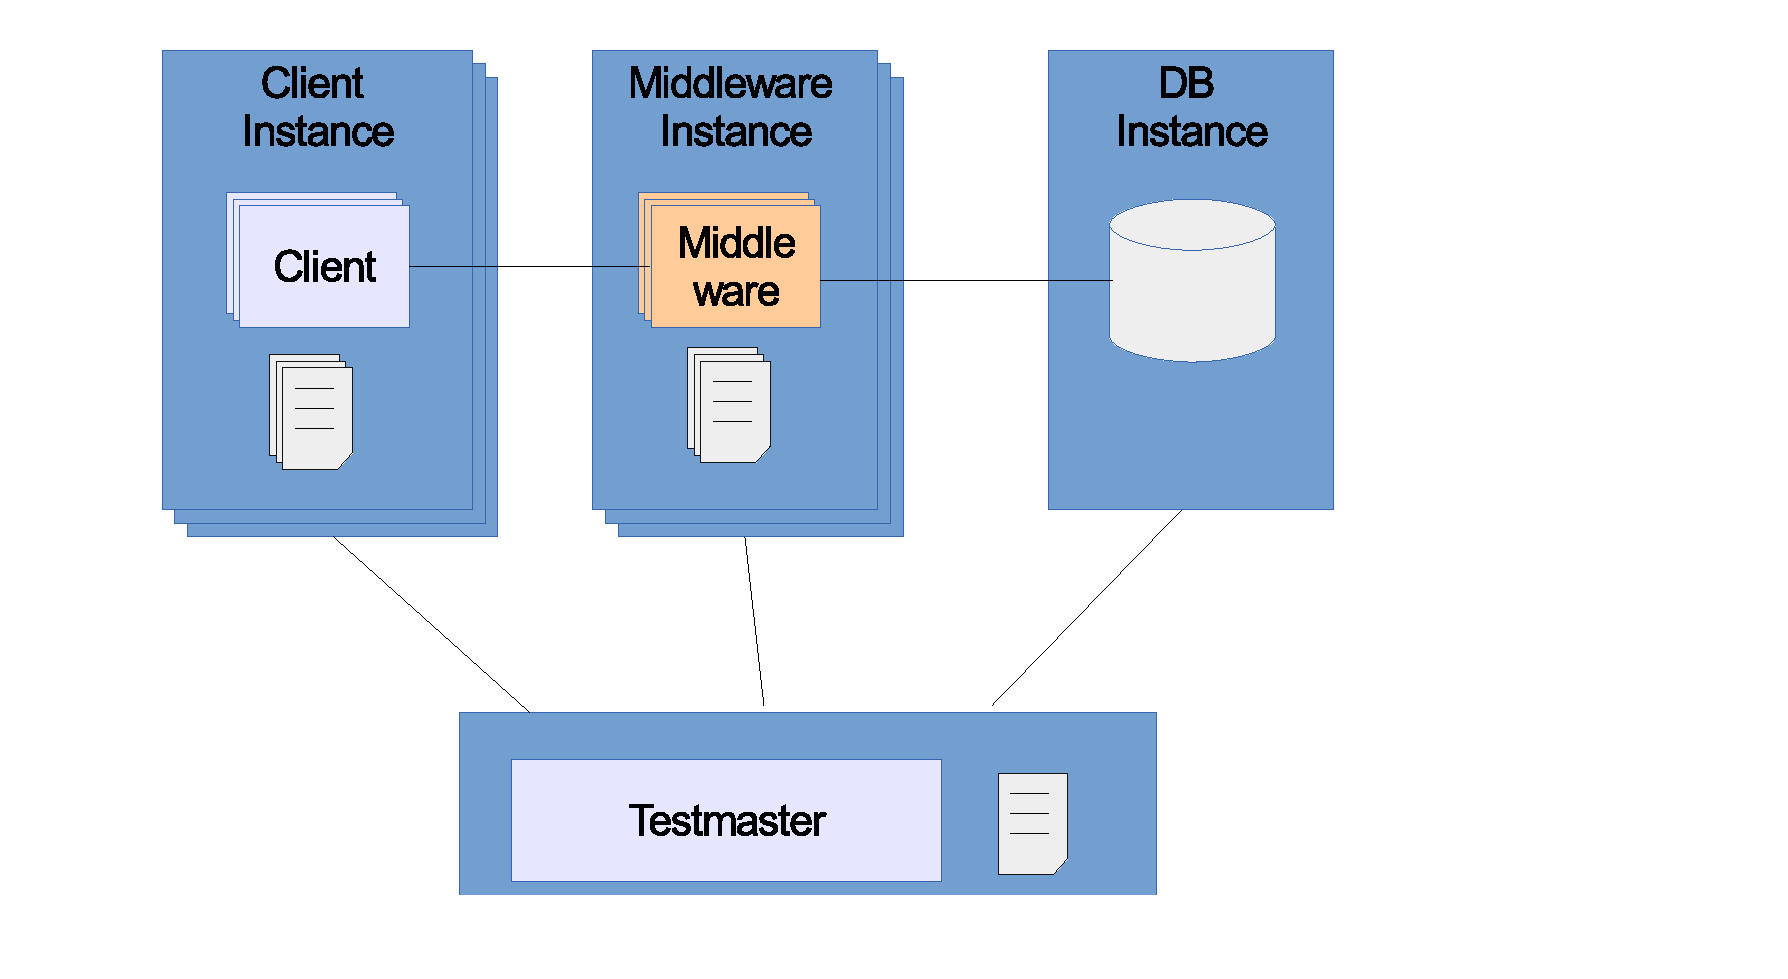
\includegraphics[scale=0.4]{../../drawings/testsystem-overview.eps}
  \end{center}
  \caption{Experiment Setup}
  \label{fig:testsystem}
\end{figure}
\end{frame}


%%%%%%%%%%% SLIDE %%%%%%%%%%%%%%%

\begin{frame}
\frametitle{TestMaster}
\begin{figure}
  \begin{center}
    \includegraphics[scale=0.3]{../../drawings/TestMaster01.png}
  \end{center}
  \label{fig:testsystem}
\end{figure}
\end{frame}


%%%%%%%%%%% SLIDE %%%%%%%%%%%%%%%

\begin{frame}
\frametitle{TestMaster}
\begin{figure}
  \begin{center}
    \includegraphics[scale=0.3]{../../drawings/TestMaster02.png}
  \end{center}
  \label{fig:testsystem}
\end{figure}
\end{frame}


%%%%%%%%%%% SLIDE %%%%%%%%%%%%%%%

\begin{frame}
\frametitle{TestMaster}
\begin{figure}
  \begin{center}
    \includegraphics[scale=0.3]{../../drawings/TestMaster03.png}
  \end{center}
  \label{fig:testsystem}
\end{figure}
\end{frame}


%%%%%%%%%%% SLIDE %%%%%%%%%%%%%%%

\begin{frame}
\frametitle{TestMaster}
\begin{figure}
  \begin{center}
    \includegraphics[scale=0.3]{../../drawings/TestMaster04.png}
  \end{center}
  \label{fig:testsystem}
\end{figure}
\end{frame}


%%%%%%%%%%% SLIDE %%%%%%%%%%%%%%%

\begin{frame}
\frametitle{TestMaster}
\begin{figure}
  \begin{center}
    \includegraphics[scale=0.3]{../../drawings/TestMaster05.png}
  \end{center}
  \label{fig:testsystem}
\end{figure}
\end{frame}


%%%%%%%%%%% SLIDE %%%%%%%%%%%%%%%

\begin{frame}
\frametitle{Memory Consumption}
2h Test with constant low load.
\begin{figure}
  \begin{center}
    \includegraphics[scale=0.3]{5clientsAt100msPerSecond.PNG}
  \end{center}
  \caption{5 Clients trying to send 100 Messages per Second}
  \label{fig:testsystem}
\end{figure}
\end{frame}

\end{document}
